% !TEX root = lecture.tex
\chapter{Sobolev Spaces and Elliptic Equations}

Sobolev spaces are fundamental in the study of partial differential equations and their
numerical approximations. In this chapter, we shall give brief discussions on the Sobolev
spaces and the regularity theory for elliptic boundary value problems.


\section{Sobolev Spaces}

We shall state and explain main results (without proofs) on Sobolev spaces. We refer to
\cite{Adams1975,Brezis2011} for comprehensive treatment.

\subsection{Preliminaries}
We first set up the environment of our discussion: Lipschitz domains,
multi-index notation for differentiation, and some basic functional spaces.


Given two metric spaces $(X, d_X)$ and $(Y, d_Y)$, where $d_X$ denotes the metric on the set $X$ and $d_Y$ is the metric on set $Y$, a function $f : X \to Y$ is called \textbf{Lipschitz continuous} if there exists a real constant $K\geq 0$ such that, for all $x_1$ and $x_2$ in $X$,
\[
d_{Y}(f(x_{1}),f(x_{2}))\leq Kd_{X}(x_{1},x_{2}).
\]

In particular, a real-valued function $f : R \to R$ is called Lipschitz continuous if there exists a positive real constant $K$ such that, for all real $x_1$ and $x_2$,
\[
|f(x_{1})-f(x_{2})|\leq K|x_{1}-x_{2}|.
\]

A domain (a connected open set) $\Omega\subset\mathbb R^n$ is called a \textbf{Lipschitz domain} if its boundary
$\partial\Omega$ can be locally represented by Lipschitz continuous function; namely for any $x\in\partial\Omega$,
there exists a neighborhood of $x$, $G\subset \mathbb R^n$, such that $G\cap\partial\Omega$ is the graph of a Lipschitz
continuous function under a proper local coordinate system.

\begin{example}
\begin{itemize}
\item All the smooth domains are Lipschitz.
\item A non-smooth example is that every polygonal domain in $\mathbb R^2$ or polyhedron in $\mathbb R^3$ is Lipschitz.
\item Every convex domain in $\mathbb R^n$ is Lipschitz.
\item A simple example of non-Lipschitz domain is two polygons touching at one vertex only.
\item A more interesting non-Lipschitz domain is a domain with cusp points on the boundary.
\end{itemize}
\end{example}
\begin{figure}[htbp]
  \centering
  % Requires \usepackage{graphicx}
  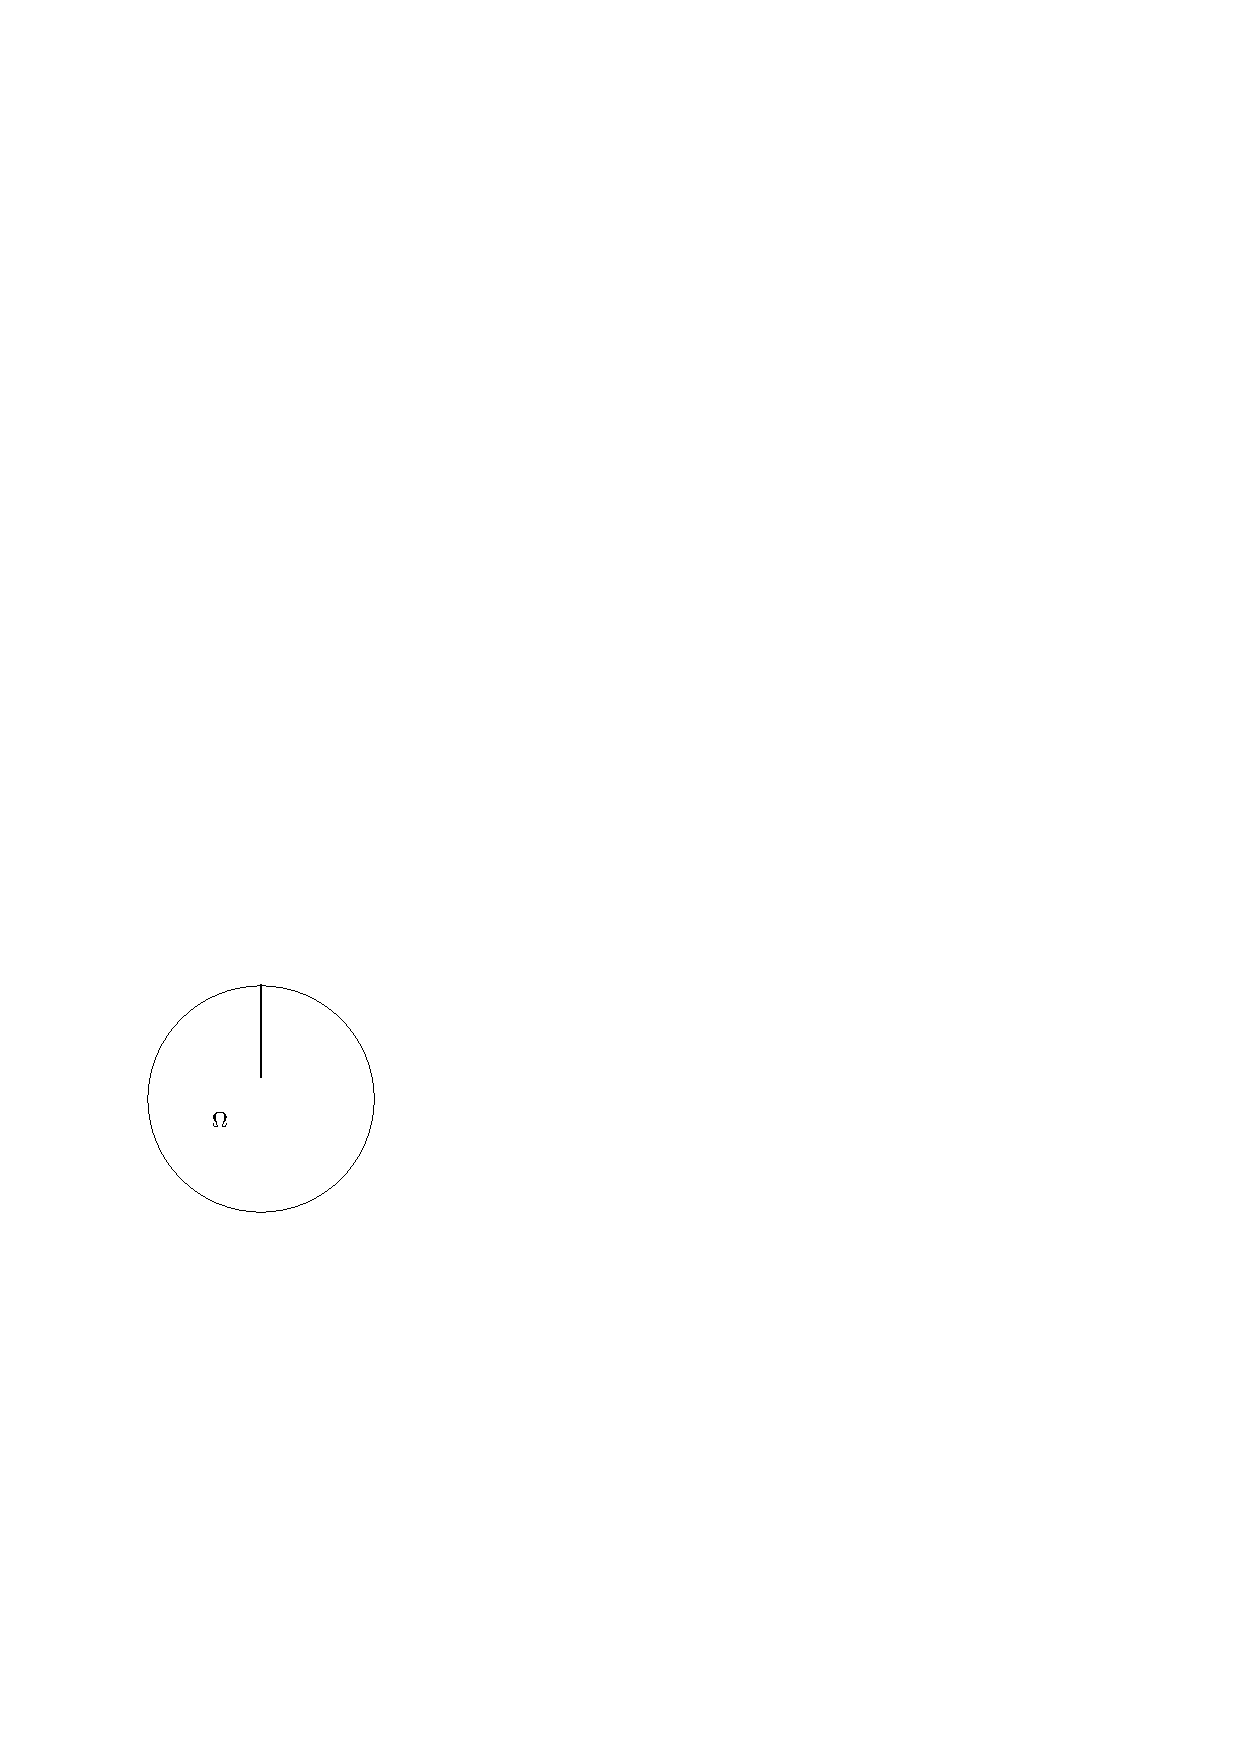
\includegraphics[width=3cm]{figures/slitdomain}\quad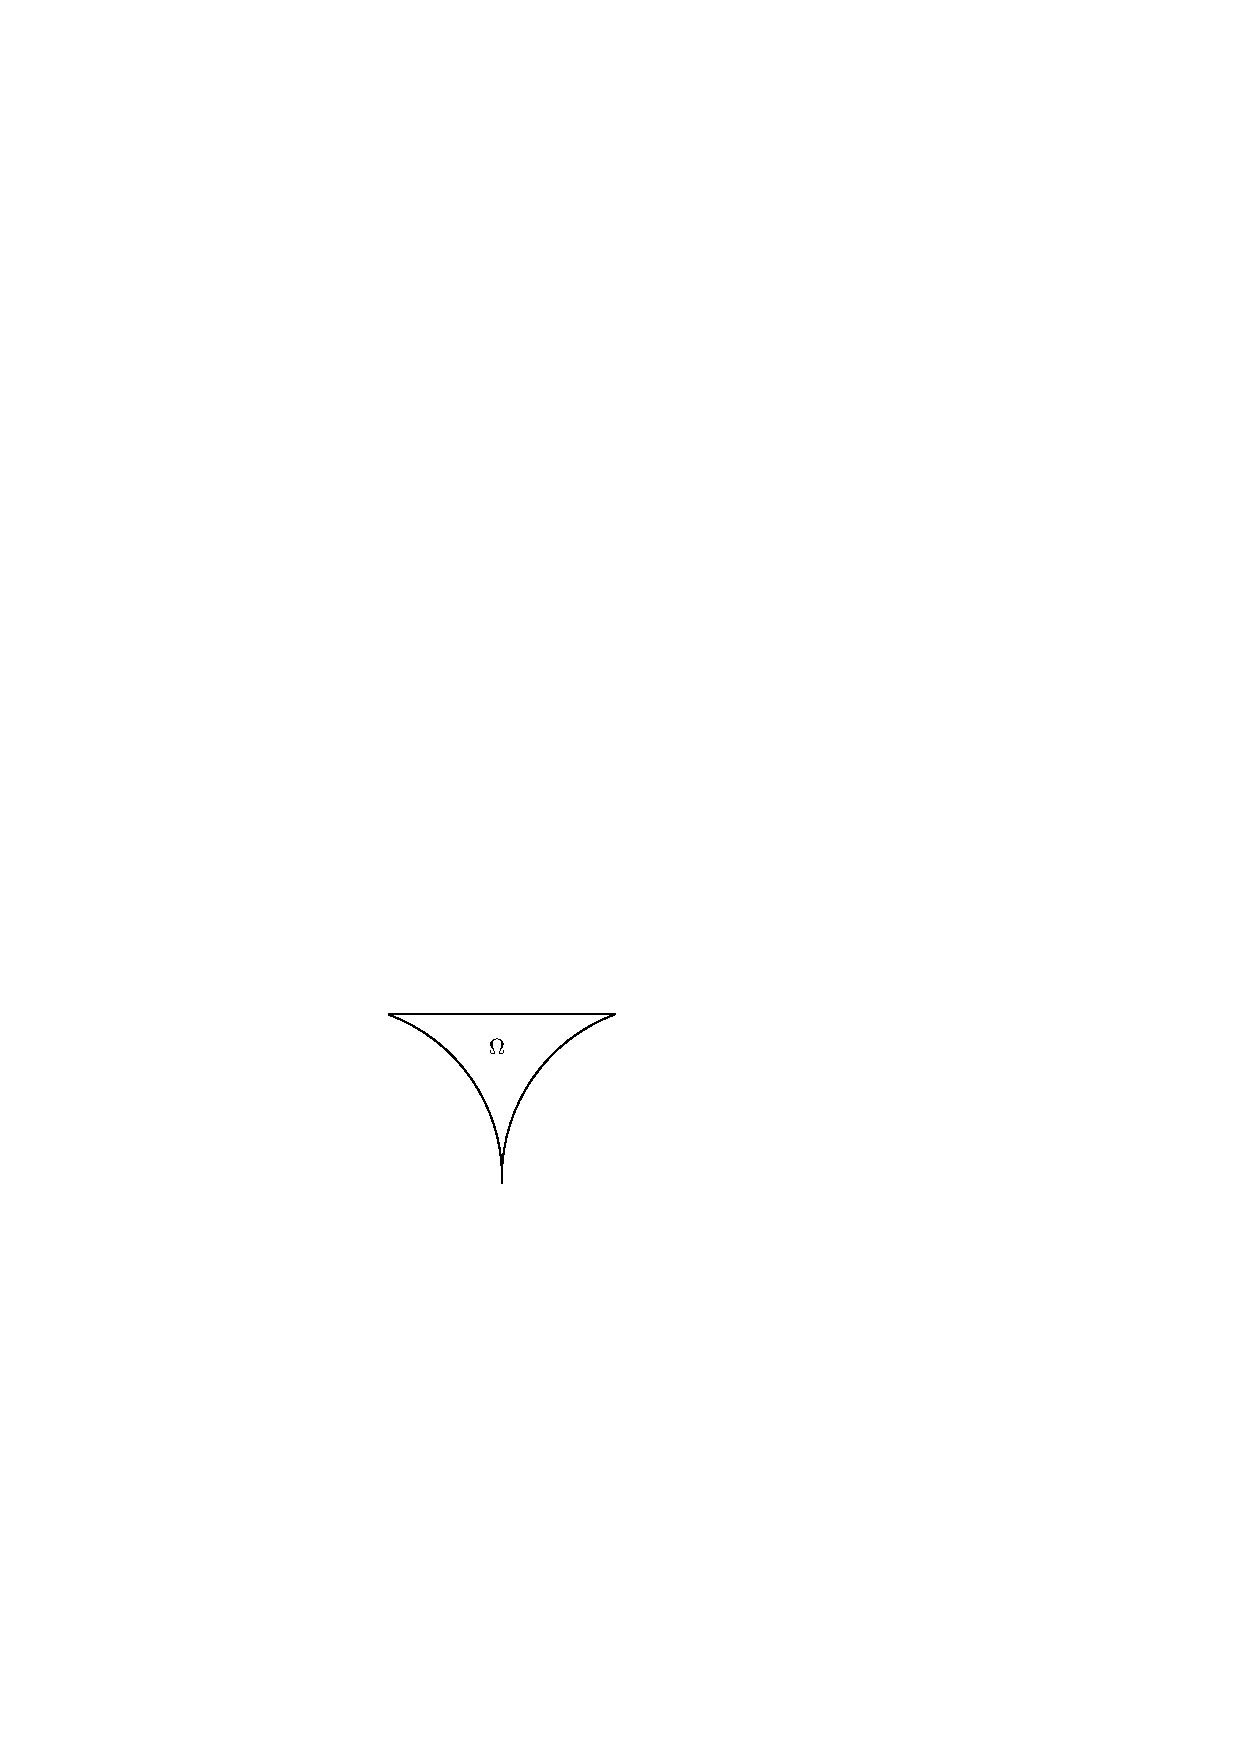
\includegraphics[width=3.5cm]{figures/cuspdomain}\\
  \caption{Domains that are not Lipschitz: slit domain (left) and cusp domain (right)}\label{nonLipschitzDmain}
\end{figure}


Let $\alpha=(\alpha_1, \cdots, \alpha_n)\in\mathbb Z_+^n$, where $\mathbb Z_+^n$ is the set of non-negative integers, be a vector
of nonnegative integers. Denote by $|\alpha|=\sum_{i=1}^n\alpha_i$. For a smooth function $v$ and $x =(x_1,  x_2, \cdots, x_n)\in\mathbb R^n$, denote
\[
D^{\alpha}v=\frac{\partial^{|\alpha|}v}{\partial x_1^{\alpha_1}\cdots\partial x_n^{\alpha_n}},\quad \textrm{and } x^{\alpha}=x_1^{\alpha_1}\cdots x_n^{\alpha_n}.
\]

Several basic Banach spaces will often be used in this book. $C(\bar{\Omega})$ is the space of continuous functions on $\bar{\Omega}$
with the usual maximum norm
\[
\|v\|_{C(\bar{\Omega})}=\max_{x\in\bar{\Omega}}|v(x)|.
\]
$C_0^{\infty}(\Omega)$ denotes the space of infinitely differential functions in $\Omega$
 that vanish in some neighborhood of $\partial\Omega$; namely $\mathrm{supp}(v)\subset\Omega$, where
 \[
 \textrm{supp}(v)=\textrm{closure of }\{x\in\Omega: v(x)\neq0\}.
 \]

A function $u$ that is measurable on $\Omega$ is said to be
\textbf{essentially bounded} on $\Omega$ if there is a constant $K$ such that $|u(x)|\leq K$ a.e. on $\Omega$.
The greatest lower bound of such constants $K$ is called the essential supremum of
$|u|$ on $\Omega$, and is denoted by $\textrm{ess}\sup_{x\in\Omega}|u(x)|$.

Given $1\leq p<\infty$, denote by $L^p(\Omega)$ the class of all measurable functions $u$ defined on
$\Omega$ for which $\int_{\Omega}|u(x)|^p\dx<\infty$, and by $L^{\infty}(\Omega)$ the vector space of all functions $u$ that are essentially bounded on $\Omega$.
The norm is defined by
\[
\|u\|_{p,\Omega}=\left(\int_{\Omega}|u|^p\dx\right)^{1/p}\quad\textrm{for }1\leq p<\infty,
\]
and
\[
\|u\|_{\infty,\Omega}=\textrm{ess}\sup_{x\in\Omega}|u(x)|.
\]

We identify in $L^p(\Omega)$ with $1\leq p\leq\infty$ functions that are equal almost everywhere in $\Omega$; the elements
of $L^p(\Omega)$ are thus equivalence classes of measurable functions satisfying $\|u\|_{p,\Omega}<\infty$, two
functions being equivalent if they are equal a.e. in $\Omega$.

\begin{exe}
Prove that $L^p(\Omega)$, $1\leq p\leq\infty$ defined above are Banach spaces.
\end{exe}


\subsection{Definition of Sobolev spaces}
The conventional way to understand a function is
through its point-wise values which is not adequate. It is better to understand a function as
a functional through its action on a space of unproblematic test functions (convential and
well-behaved functions). In this way, the concept of functions can be generalized to distributions.
``Integration by parts'' is used to extend the differentiation operators from classic
differentiable functions to distributions by shifting the operators to the test functions.
Sobolev spaces will be first defined here for integer orders using the concept of distributions
and their weak derivatives. The fractional order Sobolev spaces will be introduced
by looking at the $p$th power integrable of quotient of difference. Definitions will also be
given to Sobolev spaces satisfying certain zero boundary conditions.

\vskip0.5cm\noindent{\it Distributions and weak derivatives}.
We begin with the nice function space $C_0^{\infty}(\Omega)$. Obviously
$C_0^{\infty}(\Omega)$ is a real vector space and can be turned into a topological vector space
by a proper topology. The space $C_0^{\infty}(\Omega)$ equipped with the following topology is denoted
by $\mathcal D(\Omega)$: a sequence of functions $\{\phi_k\}\subset C_0^{\infty}(\Omega)$ is said to be convergent to a function
$\phi\in C_0^{\infty}(\Omega)$ in the space $\mathcal D(\Omega)$ if
\begin{enumerate}
\item there exists a compact set $K\subset\Omega$
 such that for all $k$, $\textrm{supp}(\phi_k-\phi) \subset K$, and
\item for every $\alpha\in\mathbb Z_+^n$, we have $\lim_{k\to\infty}D^{\alpha}\phi_k(x) = D^{\alpha}\phi(x)$ uniformly on $K$.
\end{enumerate}

The space, denoted by $\mathcal D'(\Omega)$, of all continuous linear functionals on $\mathcal D(\Omega)$ is called the (Schwarz) {\it distribution space}. The space $\mathcal D'(\Omega)$ will be equipped with the weak star
topology. Namely, in $\mathcal D'(\Omega)$, a sequence $T_n$ converge to $T$ in the distribution sense if and only if $\langle T_n, \phi\rangle\to\langle T, \phi\rangle$ for all $\phi\in\mathcal D(\Omega)$, where $\langle\cdot, \cdot\rangle: \mathcal D'(\Omega)\times \mathcal D(\Omega)\to\mathbb R$ is the
duality pair. A function $\phi$ belonging to $\mathcal D(\Omega)$ is called a {\it test function} since the action of a
distribution on $\phi$ can be thought as a test.

\begin{example}\label{exm:diracdelta}
By the definition, an element in $\mathcal D'(\Omega)$ is uniquely determined by its action.
The action could be very general and abstract as long as it is linear and continuous. As an example, let us introduce the Dirac delta distribution $\delta\in\mathcal D'(\Omega)$ with $0\in\Omega\subset\mathbb R^n$ defined
as
\[
\langle \delta, \phi\rangle = \phi(0) \quad\textrm{ for all } \phi\in \mathcal D(\Omega).
\]
\end{example}

One important class of distributions is to use the integration as the action. A function
is called {\it locally integrable} if it is Lebesgue integrable over every compact subset of $\Omega$.
We define the space $L^1_{\textrm{loc}}(\Omega)$ as the space containing all locally integrable functions. We
can embed $L^1_{\textrm{loc}}(\Omega)$ into $\mathcal D'(\Omega)$ using the integration as the duality action. For a function
$u\in L^1_{\textrm{loc}}(\Omega)$, define $T_u\in\mathcal D'(\Omega)$ as
\[
\langle T_u, \phi\rangle:=\int_{\Omega}u\phi\dx\quad \textrm{for all }\phi\in\mathcal D(\Omega).
\]
We shall still denoted $T_u$ by $u$. The correspondence $u \mapsto T_u$ is often used to identify an ``ordinary'' function as a distribution.

A distribution is often also known as a {\it generalized function} as the concept of distribution
is a more general than the concept of the classic function. One of the basic distribution
which is not an ``ordinary'' function is the Dirac $\delta$-distribution introduced in Example~\ref{exm:diracdelta}. Indeed, one motivation of the invention of distribution space is to include Dirac delta
``function''.

\begin{exe}
Prove that it is not possible to represent delta distribution by a locally integrable
function.
\end{exe}

If $u$ is a smooth function, it follows from integration by parts that, for any $\alpha\in\mathbb Z_+^n$
\[
\int_{\Omega}D^{\alpha}u(x)\phi(x)\dx=(-1)^{|\alpha|}\int_{\Omega}u(x)D^{\alpha}\phi(x)\dx\quad\textrm{for all } \phi\in\mathcal D(\Omega).
\]
There are no boundary terms, since $\phi$ has compact support in $\Omega$
 and thus $\phi$, together with
its derivatives, vanishes near $\partial\Omega$. The above identity is the basis for defining derivatives
for a distribution. If $T\in\mathcal D'(\Omega)$, then for any $\alpha\in\mathbb Z_+^n$, we define {\it weak derivative} $D^{\alpha}T$ as
the distribution given by
\[
\langle D^{\alpha}T, \phi\rangle=(-1)^{|\alpha|}\langle T, D^{\alpha}\phi\rangle\quad\textrm{for all } \phi\in\mathcal D(\Omega).
\]
It is easy to see for a differentiable function, its weak derivative coincides with its classical
derivative. But in general, the weak derivative is much weaker than the classical one such
that the differential operator can be extended from differential functions to a much larger
space: the space of distributions. For example, we can even talk about the derivative of a
discontinuous function.

\begin{example}
The Heaviside step function is defined as $S(x) = 1$ for $x > 0$ and $S(x) = 0$
for $x < 0$. By the definition
\[
\int_{\mathbb R}S'\phi\dx=-\int_{\mathbb R}S\phi'\dx=-\int_0^{\infty}\phi'\dx=\phi(0).
\]
Therefore $S'=\delta$ in the distribution sense but \textcolor[rgb]{1.00,0.00,0.00}{$\delta$ is not a function in $L_{\textrm{loc}}^1(\Omega)$}.
\end{example}

\vskip0.5cm\noindent{\it Integer order Sobolev spaces}.
The Sobolev space of index $(k, p)$, where $k$ is a nonnegative
integer and $p\geq1$, is defined by
\[
W^{k,p}(\Omega):=\{v\in L^p(\Omega): D^{\alpha}v\in L^p(\Omega)\;\textrm{  for all } |\alpha|\leq k\}
\]
with a norm $\|\cdot\|_{k,p,\Omega}$
 given by
\[
\|v\|_{k,p,\Omega}^p:=\sum_{|\alpha|\leq k}\|D^{\alpha}v\|_{0,p,\Omega}^p.
\]
We will have occasions to use the seminorm $|\cdot|_{k,p,\Omega}$
 given by
\[
|v|_{k,p,\Omega}^p:=\sum_{|\alpha|= k}\|D^{\alpha}v\|_{0,p,\Omega}^p.
\]

For $p = 2$, it is customary to write
$H^k(\Omega) := W^{k,2}(\Omega)$, which is a Hilbert space
together with an inner product as follows
\[
(u, v)_{H^k(\Omega)} =\sum_{|\alpha|\leq k}(D^{\alpha}u, D^{\alpha}v)_{L^2(\Omega)}=\sum_{|\alpha|\leq k}\int_{\Omega}D^{\alpha}uD^{\alpha}v\dx
\]
and the corresponding norm is denoted by $\|v\|_{k, \Omega}=\|v\|_{k, 2, \Omega}$.

\begin{exe}
Prove that $W^{k,p}(\Omega)$ is a Banach space.
\end{exe}

For a function in $L^{p}(\Omega)$, treating it as a distribution, its weak derivatives always exists as distributions. But the weak derivative may not be in the space $L^{p}(\Omega)$. Therefore an element in $W^{k,p}(\Omega)$ possesses certain smoothness.

\begin{example}
We consider the Heaviside function restricted to $(-1, 1)$ and still denote
by $S$. The weak derivative of $S$ is Delta distribution which is not integrable. Therefore $S \notin H^1(-1, 1)$.
\end{example}

\begin{example}
Let $u(x)=|x|$ for $x\in(-1,1)$ be an anti-derivative of $2(S-1/2)$. Obviously
$u\in L^2(-1, 1)$ and $u'\in L^2(-1, 1)$. Therefore $u\in H^1(-1, 1)$.
\end{example}


\vskip0.5cm\noindent{\it Fractional order Sobolev spaces}.
In the definition of classic derivatives, it takes the pointwise
limit of the quotient of difference. For functions in Sobolev space, we shall use the
$p$th power integrability of the quotient difference to characterize the differentiability.

For $0<\theta<1$ and $1\leq p<\infty$, we define
\[
W^{\theta, p}(\Omega)=\left\{v\in L^p(\Omega): \int_{\Omega}\int_{\Omega}\frac{|v(x)-v(y)|^p}{|x-y|^{n+\theta p}}\dx\dd y<\infty\right\}
\]
and
\[
H^{\theta}=W^{\theta, 2}(\Omega).
\]
In $W^{\theta, p}(\Omega)$, we define the following semi-norm
\begin{equation}\label{eq:fsobolevseminorm}
|v|_{\theta,p,\Omega}:=\left(\int_{\Omega}\int_{\Omega}\frac{|v(x)-v(y)|^p}{|x-y|^{n+\theta p}}\dx\dd y\right)^{1/p},
\end{equation}
and norm
\[
\|v\|_{\theta,p,\Omega}:=\left(\|v\|_{0,p,\Omega}^p+|v|_{\theta,p,\Omega}^p\right)^{1/p}.
\]

\begin{example}
For the Heaviside function S restricted to $(-1, 1)$, we look at the integral \eqref{eq:fsobolevseminorm}. To be in the space $W^{\theta, p}(\Omega)$, it is essential
to have the integral
\[
\int_0^1\frac{1}{x^{\theta p}}\dx<\infty.
\]
That is to require $\theta < 1/p$. In particular, we conclude $S\in H^{1/2-\epsilon}(-1, 1)$ for any $0 <\epsilon\leq 1/2$ but $S\notin H^{1/2}(-1, 1)$.
\end{example}

Given $s = k + \theta$ with a real number $\theta\in(0, 1)$ and an integer $k\geq0$, define
\[
W^{s,p}(\Omega):=\{v\in W^{k,p}(\Omega): D^{\alpha}v\in W^{\theta,p}(\Omega), |\alpha|= k\}.
\]
In $W^{s,p}(\Omega)$, we define the following semi-norm and norm
\[
|v|_{s,p,\Omega}=\left(\sum_{|\alpha|=k}|D^{\alpha}v|_{\theta,p,\Omega}^p\right)^{1/p}, \quad \|v\|_{s,p,\Omega}=\left(\|v\|_{k,p,\Omega}^p+|v|_{s,p,\Omega}^p\right)^{1/p}.
\]


\vskip0.5cm\noindent{\it Negative order Sobolev spaces}.
$W^{k,p}(\Omega)$ is a Banach space, i.e., it is complete in the
topology induced by the norm $\|\cdot\|_{k,p,\Omega}$. Indeed
$\{\phi\in C^{\infty}(\Omega): \|\phi\|_{k,p,\Omega}<\infty\}$ is dense in
$W^{k,p}(\Omega)$. When $\Omega$ satisfies the segment condition, $C^{\infty}(\overline{\Omega})$ is dense in
$W^{k,p}(\Omega)$ \cite{AdamsFournier2003}.
 The closure of
$C_0^{\infty}(\Omega)$ with respect to the same topology is denoted
by $W_0^{k,p}(\Omega)$. For $p = 2$, we usually write $H_0^k(\Omega) = W_0^{k,2}(\Omega)$. Roughly speaking for $u\in H_0^1(\Omega)$, $u|_{\partial \Omega}=0$ in an appropriate sense. Except $k = 0$ or
$\Omega=\mathbb R^n$, $W_0^{k,p}(\Omega)$ is a
proper subspace of $W^{k,p}(\Omega)$.

For $k\in\mathbb N$, $W^{-k,p}(\Omega)$ is defined as the dual space of $W_0^{k,p'}(\Omega)$, where $p'$ is the conjugate
of $p$, i.e., $1/p + 1/p' = 1$. In particular $H^{-k}(\Omega) = (H_0^{k}(\Omega))'$, and for $f\in H^{-k}(\Omega)$
\[
\|f\|_{-k,\Omega}=\sup_{v\in H_0^k(\Omega)}\frac{\langle f, v\rangle}{\|v\|_{k,\Omega}}.
\]

%\begin{theorem}[refs?]
%Let $v\in\mathcal D'(\Omega)$. Then $v\in W^{-k,p}(\Omega)$ if and only if
%\[
%v=\sum_{|\alpha|\leq k}D^{\alpha}v_{\alpha}\quad\textrm{for some } v_{\alpha}\in L^p(\Omega).
%\]
%\end{theorem}


\subsection{Extension theorems}
The extension theorem presented below is a fundamental result
for Sobolev spaces. Fourier transform is a powerful tool. But unfortunately it only works
for functions defined in the entire space $\mathbb R^n$. To generalize results proved on the whole $\mathbb R^n$ to a bounded domain $\Omega$, we can try to extend the function defined in $W^{k,p}(\Omega)$ to
$W^{k,p}(\mathbb R^n)$. The extension of a function $u\in L^p(\Omega)$ is trivial. For example, we can simply
set $u(x) = 0$ when $x\notin\Omega$ which is called zero extension. But such extension will create
a bad discontinuity along the boundary and thus cannot control the norm of derivatives
especially the boundary is non-smooth. The extension of Sobolev space $W^{k,p}(\Omega)$ is subtle.
We only present the result here.

\begin{theorem}\label{thm:sobolevextension}
For any bounded Lipschitz domain $\Omega$, for any $s\geq0$ and $1\leq p \leq \infty$,
there exits a linear operator $E : W^{s,p}(\Omega)\to W^{s,p}(\mathbb R^n)$ such that
\begin{enumerate}
\item $Eu|_{\Omega}= u$, and
\item $E$ is continuous. Namely there exists a constant $C(s, \Omega)$ which is increasing with respect to $s\geq0$ such that, for all $1\leq p \leq \infty$,
\[
\|Ev\|_{s,p,\mathbb R^n}\leq C(s,\Omega)\|v\|_{s,p,\Omega}\quad\textrm{for all }v\in W^{s,p}(\Omega).
\]
\end{enumerate}
\end{theorem}

Theorem \ref{thm:sobolevextension} is well-known for integer order Sobolev spaces defined on smooth domains
and the corresonding proof can be found in most text books on Sobolev spaces. But
for Lipschitz domains and especially for fractional order spaces Theorem \ref{thm:sobolevextension} is less well-known
and the the proof of the theorem for these cases is quite complicated. For integer
order Sobolev spaces on Lipschitz domains, we refer to Calder\'on \cite{Calderon1961} or Stein \cite{Stein1970}. For
factional order Sobolev spaces on Lipschitz domains, we refer to the book by McLean \cite{McLean2000}.


\subsection{Embedding theorems}
Embedding theorems of Sobolev spaces are what make the
Sobolev spaces interesting and important. The Sobolev spaces $W^{k,p}(\Omega)$ are defined using
weak derivatives. The smoothness using weak derivatives is weaker than that using classic
derivatives.

\begin{example}\label{example:20180304-1}
In two dimensions, consider the function $u(x) = \ln|\ln|x||$ when $|x| <1/e$ and $u(x) = 0$ when $|x| \geq 1/e$. It is easy to verify that $u\in H^1(\mathbb R^2)$. But $u$ is unbounded, i.e., $u\notin C(\mathbb R^2)$.
\end{example}

Sobolev embedding theorem connects ideas of smoothness using ``weak'' and ``classic''
derivatives. Roughly speaking, it says that if a function is weakly smooth enough, then it
implies certain classic smoothness with less order of smoothness.

\begin{exe}\label{exercise:20180304-1}
Prove that if $u\in W^{1,1}(0, 1)$, then $u \in L^{\infty}(0, 1)$.
\end{exe}

We now present the general embedding theorem. For two Banach spaces $B_1$ and $B_0$, we
say $B_1$ is continuously embedded into $B_0$, denoted by $B_1\hookrightarrow B_0$, if for any $u\in B_1$, it is also in $B_0$ and the embedding map is continuous, i.e., for all $u\in B_1$
\[
\|u\|_{B_0}\lesssim \|u\|_{B_1}.
\]

\begin{theorem}[General Sobolev embedding]
Let $1\leq p\leq \infty$, $k\in\mathbb Z_+$ and $\Omega$ be a
bounded Lipschitz domain in $\mathbb R^n$.


\noindent Case 1. $kp>n$
\[
W^{k,p}(\Omega)\hookrightarrow C(\bar{\Omega}).
\]

\noindent Case 2. $kp=n$
\[
W^{k,p}(\Omega)\hookrightarrow L^q(\Omega)\quad \textrm{for all } q\in[1,\infty).
\]

\quad\;\, Furthermore
\[
W^{n,1}(\Omega)\hookrightarrow C(\bar{\Omega}).
\]

\noindent Case 3. $kp<n$
\[
W^{k,p}(\Omega)\hookrightarrow L^q(\Omega)\quad \textrm{with } \frac{1}{q}=\frac{1}{p}-\frac{k}{n}.
\]
\end{theorem}

We take the following visualization of Sobolev spaces from DeVore \cite[page 93]{DeVore1998}. This
will give us a simple way to keep track of various results. We shall do this by using points
in the upper right quadrant of the plane. The $x$-axis will correspond to the $L^p$ spaces
except that $L^p$ is identified with $x = 1/p$ not with $x = p$. The $y$-axis will correspond
to the order of smoothness. For example, the point $(1/p, k)$ represents the Sobolve space
$W^{k,p}(\Omega)$. The line with slope $n$ (the dimension of Euclidean spaces) passing through
$(1/p, 0)$ is the demarcation line for embeddings of Sobolev spaces into $L^p(\Omega)$ (see Figure~\ref{fig:sobolevEmbeddingLine}). Any Sobolev space with indices corresponding to a point above that line is embedded
into $L^p(\Omega)$ and space below that line cannot be embedded into $L^p(\Omega)$.
\begin{figure}[htbp]
  \centering
  % Requires \usepackage{graphicx}
  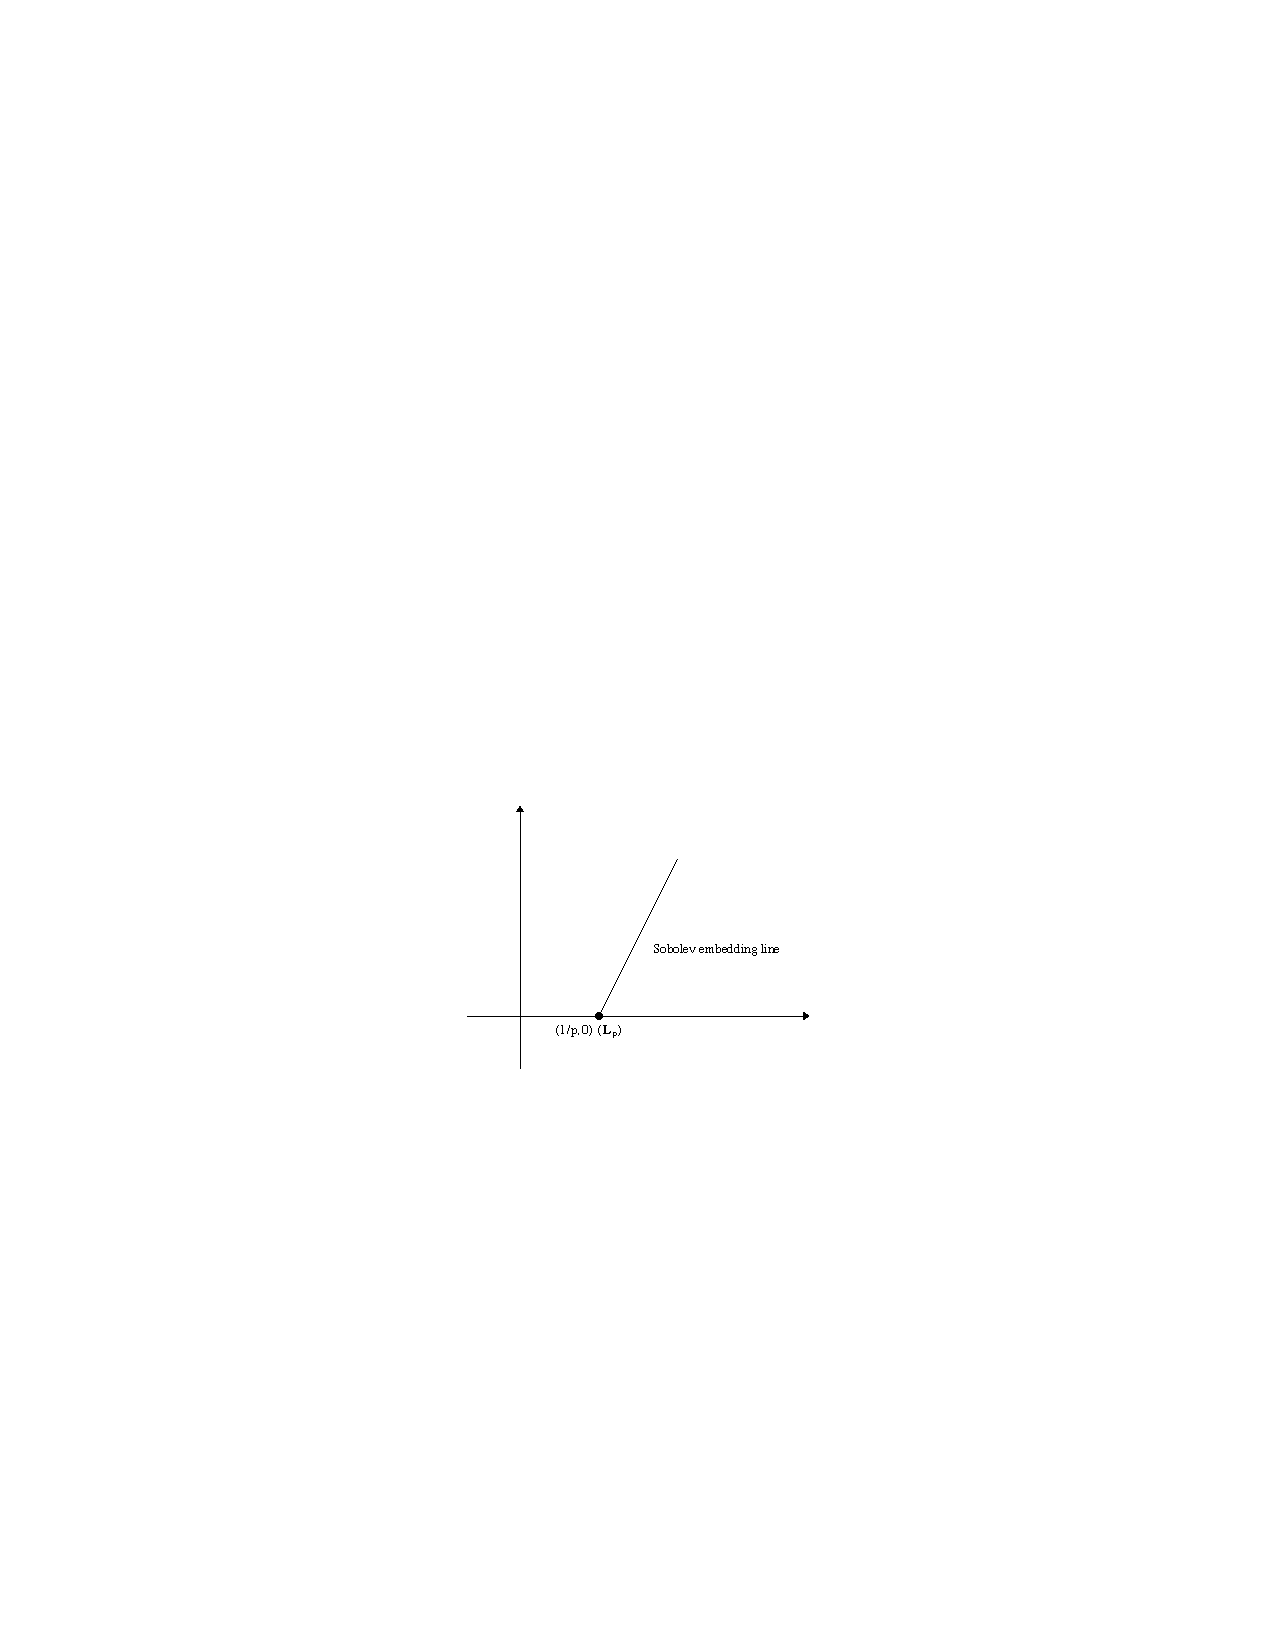
\includegraphics[width=7cm]{figures/sobolevEmbeddingLine}\\
  \caption{Sobolev embedding line}\label{fig:sobolevEmbeddingLine}
\end{figure}

To be quickly determine if a point lies above the demarcation line or not, we introduce
the {\it Sobolev number}
\[
\textrm{sob}_n(k, p)=k-\frac{n}{p}.
\]
If $\textrm{sob}_n(k, p) > 0$, functions from $W^{k,p}(\Omega)$ are continuous (or more precisely can find a
continuous representative in its equivalent class). In general
\[
W^{k,p}(\Omega)\hookrightarrow W^{l,q}(\Omega)\quad\textrm{if } k>l \textrm{ and } \textrm{sob}_n(k, p)>\textrm{sob}_n(l, q).
\]
Sobolev spaces corresponding to points on the demarcation line may or may not be
embedded in $L^p(\Omega)$. For example, for $n\geq1$
\[
W^{n,1}(\Omega)\hookrightarrow L^{\infty}(\Omega)\quad \textrm{but } W^{1,n}(\Omega)\not\hookrightarrow L^{\infty}(\Omega).
\]
Note that $W^{1,n}(\Omega)\hookrightarrow L^{p}(\Omega)$ for all $1\leq p < \infty$. Furthermore there exists a constant
$C(n, \Omega)$ depending on the dimension of Euclidean space and the Lipschitz domain such
that
\begin{equation*}
\|v\|_{0,p,\Omega}\leq C(n, \Omega)p^{1-1/n} \|v\|_{1,n,\Omega}\quad\textrm{for all }1\leq p < \infty.
\end{equation*}

\begin{example}
By the emebedding theorem, we have
\begin{enumerate}
\item $H^1(\Omega)\hookrightarrow C(\bar{\Omega})$ in one dimension (Exercise~\ref{exercise:20180304-1}).
\item $H^1(\Omega)\not\hookrightarrow C(\bar{\Omega})$ for $n\geq2$ (Example~\ref{example:20180304-1}).
Namely there is no continuous representation of a function in $H^1(\Omega)$ for $n\geq2$ and thus its point-wise value is
not well defined.
\item In 2-D, $H^1(\Omega)\hookrightarrow L^p(\Omega)$ for any $1\leq p<\infty$; in 3-D, $H^1(\Omega)\hookrightarrow L^p(\Omega)$ for any $1\leq p\leq6$.
\end{enumerate}
\end{example}


\subsection{Trace Theorem}
The trace theorem is to define function values on the boundary. If
$u\in C(\bar{\Omega})$, then $u(x)$ is well defined for $x\in\partial\Omega$. But for $u\in W^{k,p}(\Omega)$, the function
is indeed defined as an equivalent class of Lebesgue integrable functions, i.e., $u \sim v$ if
and only if $u = v$ almost everywhere. The boundary $\partial\Omega$ is a measure zero set (in $n$th
dimensional Lebesgue measure) and thus the pointwise value of $u|_{\partial\Omega}$ is not well defined
for functions in Sobolev spaces.

\begin{theorem}
Let $\Omega\subset\mathbb R^n$ be a bounded domain with smooth or Lipschitz boundary
$\Gamma=\partial\Omega$. Then the trace operator $\gamma: C^1(\bar{\Omega})\to C(\Gamma)$
 can be continuously extended to
$\gamma: H^1(\Omega)\to H^{1/2}(\Gamma)$, i.e., the trace inequality holds:
\[
\|\gamma(u)\|_{1/2, \Gamma}\lesssim \|u\|_{1, \Omega}\quad \textrm{for all } u\in H^1(\Omega).
\]
Furthermore the trace operator is surjective and has a continuous right inverse.
\end{theorem}

More general, if $\Omega$ is a Lipschitz domain, then the trace operator
$\gamma: H^s(\Omega)\to H^{s-1/2}(\Gamma)$ is bounded for $1/2 < s < 3/2$. See McLean \cite[pages 100-106]{McLean2000}.


\begin{theorem}
Suppose that $\Omega\subset\mathbb R^n$ has a Lipschitz boundary, and that $p$ is a real number in the range $1\leq p\leq \infty$. Then there is a constant $C$ such that
\[
\|v\|_{0, p,\partial\Omega}\leq C\|v\|_{0,p,\Omega}^{1-1/p}\|v\|_{1,p,\Omega}^{1/p}\quad\forall~v\in W^{1,p}(\Omega).
\]
\end{theorem}




\subsection{Norm Equivalence Theorem}
The definition of norm $\|\cdot\|_{k+1,p}$ involves all the $i$th
derivatives for $i\leq k + 1$. But the highest one is the critical one. That is we can prove \cite[Theorem 5.2 in page 135]{AdamsFournier2003}
\[
\|u\|_{k+1,p}\eqsim\|u\|_{0,p}+|u|_{k+1,p}\quad\textrm{for all } u\in W^{k+1, p}(\Omega).
\]

\begin{theorem}[Sobolev norm equivalence]
Let $P_k(\Omega)$($k\geq0$) be the set of all polynomials in $\Omega$ with the total degree no more than $k$. Let $N=\mathrm{dim}P_k(\Omega)$. Assume $f_i\in(W^{k+1,p}(\Omega))'$, $i=1,2,\cdots,N$, $p\in[1,\infty]$ such that for $q\in P_k(\Omega)$, $q=0$ if $f_i(q)=0$ for all $1\leq i\leq N$. Then
\begin{equation}\label{eq:sobolevnormequiv}
\|v\|_{k+1,p,\Omega}\lesssim  |v|_{k+1,p,\Omega}+\sum_{i=1}^N|f_i(v)|\quad\textrm{for all } v\in W^{k+1,p}(\Omega).
\end{equation}
\end{theorem}

As a special case of the Sobolev norm equivalence theorem, we present the following
variants of Poincar\'e or Friedrichs inequalities. Assume that $\Gamma$ is a measurable subset of
$\Omega$ with positive measure (in $n-1$ dimensional Lebesgue measure). Choosing $f_0(v) =\int_{\Gamma}v\dd s$
 in \eqref{eq:sobolevnormequiv}, we obtain the Friedrichs inequality
\[
\|v\|_{1,p,\Omega}\lesssim  |v|_{1,p,\Omega}+\left|\int_{\Gamma}v\dd s\right|\quad\textrm{for all } v\in W^{1,p}(\Omega).
\]
Consequently, we have the Poincar\'e inequality
\begin{equation}\label{eq:poincareinequalityW1p}
\|v\|_{1,p,\Omega}\lesssim  |v|_{1,p,\Omega}\quad\textrm{for all } v\in W_0^{1,p}(\Omega).
\end{equation}
Choosing $f_0(v)=\int_{\Omega}v\dx$, we obtain the Poincar\'e-Friedrichs inequality
\[
\|v\|_{1,p,\Omega}\lesssim  |v|_{1,p,\Omega}+\left|\int_{\Omega}v\dx\right|\quad\textrm{for all } v\in W^{1,p}(\Omega).
\]
Consequently, let $\bar{v} =\int_{\Omega}v\dx/|\Omega|$ denote the average of $v$ over $\Omega$, we get the averaged
Poincar\'e inequality
\[
\|v-\bar{v}\|_{1,p,\Omega}\lesssim  |v|_{1,p,\Omega}\quad\textrm{for all } v\in W^{1,p}(\Omega).
\]

\begin{theorem}\label{thm:quotientspacenorms}
Let $k\geq0$ and $p\in[1, \infty]$. Then
\[
\inf_{q\in P_k(\Omega)}\|v+q\|_{k+1,p,\Omega}\lesssim  |v|_{k+1,p,\Omega}\quad\textrm{for all } v\in W^{k+1,p}(\Omega),
\]
\[
\|\dot{v}\|_{k+1,p,\Omega}\lesssim  |\dot{v}|_{k+1,p,\Omega}\quad\textrm{for all } v\in W^{k+1,p}(\Omega)/P_k(\Omega).
\]
\end{theorem}


All constants hidden in the notation $\lesssim$ depends on the size and shape of the domain
$\Omega$. This is important when apply them to one simplex with diameter $h$ in finite element
methods.

\subsection{Green's formulas}
Let $\nu=(\nu_1, \nu_2, \cdots, \nu_n)$ be the unit outward normal to $\partial\Omega$.
The (outer) normal derivative operator
\[
\partial_{\nu}=\sum_{i=1}^n\nu_i\partial_i
\]
is defined almost everywhere along $\partial\Omega$ for smooth functions.
Given two functions $u, v\in H^1(\Omega)$, the following fundamental Green's formula
\[
\int_{\Omega}u\partial_iv\dx=-\int_{\Omega}\partial_iuv\dx+\int_{\partial\Omega}uv\nu_i\dd s
\]
holds for any $i=1, \cdots, n$.
From this formula, other Green's formulas may be easily deduced.
For example, replacing $u$ by $\partial_iu$ and taking the sum from $1$ to $n$, we get
\[
\int_{\Omega}\sum_{i=1}^n\partial_iu\partial_iv\dx=-\int_{\Omega}\Delta uv\dx+\int_{\partial\Omega}\partial_{\nu}uv\dd s
\]
for all $u\in H^2(\Omega)$ and $v\in H^1(\Omega)$. As a consequence, we obtain by subtraction
\[
\int_{\Omega}(u\Delta v-\Delta uv)\dx=\int_{\partial\Omega}(u\partial_{\nu}v-\partial_{\nu}uv)\dd s
\]
for all $u\in H^2(\Omega)$ and $v\in H^2(\Omega)$.


\begin{theorem}
Let $m$ be a positive integer. Let $\Omega$, $\Omega_1$ and $\Omega_2$ be three open and bounded domains in $\mathbb R^n$. Suppose
$\bar{\Omega}=\bar{\Omega}_1\cup \bar{\Omega}_2$ and $\Omega_1\cap \Omega_2=\varnothing$. Let $u$ be a function defined in
$\Omega$ such that $u|_{\Omega_1}\in C^{m-1}(\bar{\Omega}_1)\cap H^m(\Omega_1)$ and $u|_{\Omega_2}\in C^{m-1}(\bar{\Omega}_2)\cap H^m(\Omega_2)$.
Then $u\in H^m(\Omega)$ if and only if $u\in C^{m-1}(\bar{\Omega})$.
\end{theorem}
For a piecewise smooth function which is also in $H^1(\Omega)$, then it is globally continuous.
\begin{exe}
Let $\Omega$, $\Omega_1$ and $\Omega_2$ are three open and bounded domains in $\mathbb R^n$. Suppose
$\bar{\Omega}=\bar{\Omega}_1\cup \bar{\Omega}_2$ and $\Omega_1\cap \Omega_2=\varnothing$. Let $u$ be a function defined in
$\Omega$ such that $u|_{\Omega_1}\in C(\bar{\Omega}_1)\cap H^1(\Omega_1)$ and $u|_{\Omega_2}\in C(\bar{\Omega}_2)\cap H^1(\Omega_2)$.
Prove that $u\in H^1(\Omega)$ if and only if $u\in C(\bar{\Omega})$.
\end{exe}



\section{Elliptic Boundary Value Problems and Regularity}

\subsection{Weak formulation}
Let us take the Poisson equation with homogenous Dirichlet
boundary condition
\begin{equation}\label{eq:poisson}
-\Delta u=f\;\; \textrm{in }\Omega, \quad \textrm{and } u|_{\partial\Omega}=0,
\end{equation}
as an example to illustrate the main idea. If there exists a function $u\in C_0^2(\Omega)$
satisfying the Poisson equation, we call $u$ a {\it classic solution}. The smoothness of $u$ excludes
many interesting solutions for physical problems. We need to seek a weak solution in more
broader spaces: Sobolev spaces. Here ``weak'' means the smoothness is imposed by weak
derivatives.

Recall the basic idea of Sobolev space is to treat function as functional. Let us try to
understand the equation \eqref{eq:poisson} in the distribution sense. We seek a solution $u\in \mathcal D'(\Omega)$ such
that for any $\phi\in C_0^{\infty}(\Omega)$,
\[
\langle-\nabla\cdot\nabla u,\phi\rangle:=\langle\nabla u,\nabla\phi\rangle=\langle f, \phi\rangle,
\]
which suggests a weak formulation: find $u\in H_0^1(\Omega)$ such that
\begin{equation}\label{eq:poissonweak}
\int_{\Omega}\nabla u\cdot\nabla v\dx=\int_{\Omega}f v\dx\quad\textrm{for all } v\in H_0^1(\Omega).
\end{equation}
And we can take $f\in H^{-1}(\Omega):=(H_0^1(\Omega))'$.

A generalization of weak formulation \eqref{eq:poissonweak} is: given an $f\in V'$ and a continuous bilinear form $a(\cdot, \cdot): U\times V\to \mathbb R$,  find a solution $u\in U$ such that
\begin{equation*}
a(u, v)=\langle f, v\rangle\quad\textrm{for all } v\in V.
\end{equation*}
Here the space $U$ is the one we seek a solution and thus called {\it trial space}, and $V$ is still
called {\it test space}.


\subsection{Regularity theory}

The weak solution $u$ of \eqref{eq:poissonweak} can be proved to be a solution of \eqref{eq:poisson} in a
more classic sense if $u$ is smooth enough such that we can integration by parts back. The
theory for proving the smoothness of the weak solution is called {\it regularity} theory, which
is the bridge to connect classical and weak solutions.

First we assume right hand side $f\in L^2(\Omega)$ which will imply $\Delta u\in L^2(\Omega)$.
\begin{theorem}
Let $u$ be the solution of \eqref{eq:poissonweak}. If $f\in L^2(\Omega)$, then $-\Delta u = f$ in $L^2(\Omega)$, i.e.
\begin{equation}\label{eq:equilibriumweak}
\int_{\Omega}-\Delta u \,v\dx=\int_{\Omega}fv\dx\quad\forall~v\in L^2(\Omega).
\end{equation}
Furthermore $u = 0$ on $\partial\Omega$ in the trace sense.
\end{theorem}
\begin{proof}
When $f\in L^2(\Omega)$, $\langle f, v\rangle = (f, v)$. Choosing $v\in C_0^{\infty}(\Omega)\subset H_0^1(\Omega)$ in \eqref{eq:poissonweak} implies that
\[
\langle-\Delta u, v\rangle = (f, v)\quad\forall~v\in C_0^{\infty}(\Omega).
\]
That is $-\Delta u$ as a distribution is equal to $f\in L^2(\Omega)$. Since $C_0^{\infty}(\Omega)$ is dense in $L^2(\Omega)$ and
both sides are continuous in $L^2$ topology, we conclude \eqref{eq:equilibriumweak}.
\end{proof}

\begin{theorem}[\cite{Evans2010}]\label{thm:poissonregularitysmooth}
Let $\Omega$ be a smooth and bounded domain of $\mathbb R^n$. Then for each $f \in L^2(\Omega)$,
there exists a unique $u\in H^2(\Omega)$, the solution of \eqref{eq:poissonweak}, that satisfies
\[
\|u\|_{2,\Omega}\leq C\|f\|_{0,\Omega}
\]
where $C$ is a positive constant depending on $\Omega$.
\end{theorem}

Theorem~\ref{thm:poissonregularitysmooth}, however, does not hold on general Lipschitz domains.
The requirement of $\Omega$ is necessary. When $\partial\Omega$ is only Lipschitz continuous, we may not
be able to glue boundary pieces on the corner points. This is not only a technical difficulty.
We now give an example in which the regularity of $u$ depends on the shape of $\Omega$.
\begin{example}
Let us give a simple counter example. Given $\beta\in (0, 1)$, consider the
following nonconvex domain
\[
\Omega=\{(r, \theta): 0<r<1, 0<\theta<\pi/\beta\}.
\]
Let $v = r^{\beta}\sin(\beta\theta)$. Being the imaginary part of the complex analytic function $z^{\beta}$, $v$ is
harmonic in $\Omega$. Define $u = (1-r^2)v$. A direct calculation shows that
\[
-\Delta u=4(1+\beta)v\quad\textrm{  in }\Omega,\quad\textrm{and } u|_{\partial\Omega}=0.
\]
Note that $4(1+\beta)v\in L^{\infty}(\Omega)\subset L^2(\Omega)$, but $u\notin H^2(\Omega)$.
\end{example}

Nevertheless, a slightly weaker result does hold for general Lipschitz domains.
\begin{theorem}[\cite{Dauge1988,BacutaBrambleXu2003}]
Assume that $\Omega$ is a bounded Lipschitz domain. Then there exists a constant
$\alpha\in(0, 1]$ such that
\[
\|u\|_{1+\alpha,\Omega}\leq C\|f\|_{\alpha-1,\Omega}
\]
for the solution $u$ of \eqref{eq:poissonweak},
where $C$ is a constant depending on the domain $\Omega$.
\end{theorem}

A remarkable fact is that we can take $\alpha = 1$ in the above theorem for
convex domains. This means that Theorem~\ref{thm:poissonregularitysmooth} can be extended to convex domains.
\begin{theorem}\label{thm:poissonregularityconvex}
Let $\Omega$ be a convex, bounded domain of $\mathbb R^n$. Then for each $f \in L^2(\Omega)$,
there exists a unique $u\in H^2(\Omega)$, the solution of \eqref{eq:poissonweak}, that satisfies
\[
\|u\|_{2,\Omega}\leq C\|f\|_{0,\Omega}
\]
where $C$ is a positive constant depending on $\Omega$.
\end{theorem}

When $\Omega$ is a concave polygon in $\mathbb R^2$, we do not have full regularity, i.e.,
$\alpha < 1$. There are at least two ways to obtain analogous (but weaker) results for concave
domain. The first one (see \cite{Dauge1988,BacutaBrambleXu2003}) is to use fractional Sobolev spaces: namely $-\Delta$:
$H_0^1(\Omega)\cap H^{1+s}(\Omega)\to H^{-1+s}(\Omega)$ which holds for any $s\in [0, s_0)$ for some $s_0\in (0, 1]$
depending on $\Omega$.

Another approach is to use $L^p$ space, instead of $L^2$. It can be shown that (cf. \cite{Grisvard1985})
\[
-\Delta: H_0^1(\Omega)\cap W^{2,p}(\Omega)\to L^{p}(\Omega)
\]
is an isomorphism, which holds for any $p\in(1, p_0)$ for some $p_0 > 1$ that depends on the domain $\Omega$.
